\chapter{Related Work}\label{chap:related}
In this chapter, we explore existing literature, research, and data collected prior to our work that serve as basis for this thesis. By reviewing the related work we aim to develop an understanding of the current state of research and want to position our work within the broader context of metadata extraction in scholarly literature.\\
More precisely, we review academic literature related to the topic of metadata extraction in scholarly work.\\
Our exploration also encompasses an examination of existing software solutions, related to our problem. We analyze the methodologies employed by these software applications, studying their approaches, techniques, and involved data.\\
Furthermore, we examine relevant datasets, which are connected to this issue and can be utilized as basis for our own model development.\\
To provide a concise overview, we categorize the related work into four categories: literature, literature accompanied by available code, software applications, and datasets.

\section{Literature}
Metadata extraction from scientific publications is a widely recognized research challenge that has garnered considerable attention over the years. Numerous approaches have been proposed to address this problem, encompassing techniques such as regular expressions, template matching, knowledge bases, and supervised ML.\\
While the majority of approaches adopt supervised ML to extract metadata from references and document header, some researchers have proposed alternative methods to retrieve this data~\cite{tkaczyk2018machine}.\par
Gupta et al.~\cite{gupta2009new}, for example, adopt a sequential methodology in their approach. Initially, they classify paragraphs by utilizing a probabilistic model that incorporates both statistic-based and lexical-based features. Subsequently, for the extraction of reference strings, they employ a template matching technique combined with regular expressions to identify and extract relevant entities. In cases where this matching fails, a knowledge-based approach is employed to search for publications. Finally, a further rule-based approach is implemented to extract entities, completing the sequential process outlined by the authors.\par
Cortez et al.~\cite{cortez2009flexible} introduce FLUX-CiM, a novel method for extracting various components from reference strings, including author names, article titles, venues, and page numbers. Their approach utilizes a knowledge base automatically constructed from existing metadata records in a specific field (e.g., computer science, health sciences, social sciences) which are commonly accessible through public data repositories or the web. They report precision and recall levels exceeding 94\% across all entities.\par
For supervised ML the most common method to extract metadata from reference strings utilizes CRF, including Zhang et al.~\cite{zhang2011parsing}, who extract the content of a reference string using a CRF model. They collect in the domain of medicine from the PubMed Central archive, which offers machine-readable XML files with structured metadata. They report a F1-score of 97,95\% on their dataset.\par
Matsuoka et al.~\cite{matsuoka2016examination}, also utilizes a CRF model to extract metadata from reference strings. They examine, which features are best suited for their task at hand and conclude that lexical features showed the most promising results.\par
The Deep Learning approach, suggested by Rizvi et al.~\cite{rizvi2020hybrid} used their handcrafted dataset to fine-tune a Mask R-CNN model for reference extraction. Their approach, called DeepBiRD, draws inspiration from human visual perception and utilizes layout characteristics to identify and distinguish individual references within a scientific publication. They report an AP50 of 98.56\% on the newly created dataset.\par
Voskuil et al.~\cite{voskuil2021improving} investigate metadata extraction from references in patents. They examine the performance of various fine-tuned BERT models on their dataset and compare it with a CRF model and Flair~\cite{akbik2019flair}. They note that the BERT models outperforms both reference models with a reported precision of 97\%.

\section{Literature with Code}\label{sec:literature_code}
\textit{EXParser}~\cite{excite_methods} is part of the EXCITE toolchain~\cite{excite_toolchain}, an application stack designed to extract and segment reference strings from scientific literature.\\
\textit{EXParser} is used in this process to extract and segment reference strings from scientific literature. The authors propose a sequential approach, employing two different models and different tasks. A Random Forests~\cite{breiman2001random} model is utilized to classify each line of a document.\\
The classification scheme employed by the researchers involves the differentiation of instances into four distinct class labels: None, representing instances that do not pertain to a reference line; first line of a reference, denoting the initial line of a reference entry; intermediate line, signifying lines within the reference entry but not the first or last line; and last reference line, indicating the final line of a reference entry.\\
Reference strings are then created from classified lines and passed forward to a CRF model, segmenting each reference into components like author, title, year, etc. The authors note that the result of the CRF segmentation model is highly dependent on the quality of the output produced by the extraction model.\\
A wide range of features is utilized by both models, consisting of format-based, lexical, semantic, and shape-based features.\\
As next step they estimate the completeness of a reference by calculating the probability density function over a set of segmented reference strings. During model inference, a filtering process to smooth the output of the line classification process is additionally applied.\\
The approach presented by the authors assumes that references are always separated from each other by line breaks. It is, however worth noting that our corpus contains various short articles, where references are not always divided by line breaks, challenging this assumption.\\
In these cases, the segmentation model can produce faulty and unusable output, if for example the author of a new reference is located on the last line of a previous reference.\\
Another concern of the line classification model might be, that no information about previous or subsequent lines is provided as feature in the training process.\par
\textit{GROBID} (\textbf{G}ene\textbf{R}ation \textbf{O}f \textbf{BI}bliographic \textbf{D}ata)~\cite{GROBID_pref} is a software tool to extract and parse technical and scientific documents from PDF files in machine-readable XML/TEI files.\\
The author utilizes a cascading structure of sequence labeling models to extract metadata like header information, bibliographic references, and structural information documents. This modular approach has the advantage, that training data, features, and even whole models can be replaced or adapted.\\
Since all models are trained with their corresponding parts of the dataset, each particular model can be trained on only a few class labels. Due to the modular cascading approach, the combined number of leaf labels amounts to 55 individual labels after the input is processed.\\
An user can freely swap between various models, but the authors suggest to use the CRF or BiLSTM-CRF model~\cite{chen2017improving}.\\
The segmentation model relies mostly on layout features and utilizes line classification to segment the document in labels like title, header, body, and bibliography. It can be considered as root model, since it processes the raw and its output is distributed to corresponding models downstream, namely the header, reference-segmenter, and fulltext model.\\
In contrast to the root model, the header model utilizes token-level classification and extracts, as its name suggests, header metadata like title, author, affiliation, and abstract.\\
The reference-segmenter model slices blocks of reference lines in individual references, which are consequently fed into the reference model, enabling the extraction of vital metadata such as authorship, title, and publication year. Year labels from the header model and reference model are further processed to extract an ISO-format for the date.\\
Labels identified as author by the header and reference model are parsed separately by the name-header and name-citation model, respectively.\\
While the authors state, they induce noise in the training data of each model to account for errors in upstream models, they acknowledge that these inaccuracies can propagate through various layers. To extract the author name from a reference, for example, the data has to pass through four different models, where each layer subsequently increases the risk of a miss-classification.\\
An outline of the structure of all cascading models of GROBID can be seen in Figure~\ref{fig:grobid}.\par

\begin{figure}[!th]
	\centering
	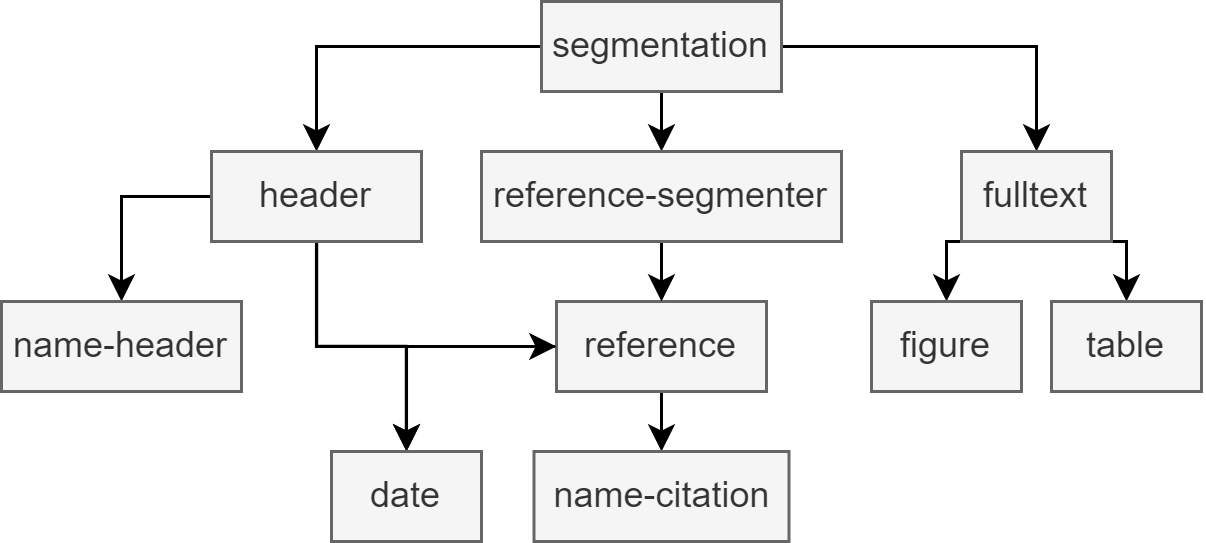
\includegraphics[width=0.7\linewidth]{images/grobid.png}
	\caption{The cascading structure of all GROBID models.}
	\label{fig:grobid}
\end{figure}

\textit{CERMINE} is an extraction system, capable of retrieving header metadata as well as reference metadata from PDF files. Similar to \textit{EXCITE} and \textit{GROBID}, the authors suggest a cascading approach using a series of different supervised and unsupervised models to enhance the performance and robustness of the overall system, allowing for more comprehensive and reliable results.\\
The extraction process starts with a layout analysis to create a hierarchical representation of a document, preserving its text content and layout features. 
Once individual characters have been retrieved, they are combined into cohesive words, followed by the assembly of lines, and ultimately integrated into zones.\\
To classify each zone accurately, a Support Vector Machine (SVM)~\cite{hearst1998support} model is employed, distinguishing between four distinct categories: metadata, body, reference, and other. 
Following the initial zone classification, a subsequent SVM model is employed to further categorize the identified zones, labeled as metadata, into distinct classes such as author zones, title zones, abstract zones, and other relevant labels.\\
Both classifiers use a wide range of geometric-based, lexical-based, sequential-based, and heuristics-based set of features. After the feature selection, the number of features is reduced to 53 and 51 features for the SVM models.\\
For the bibliography extraction, the authors employ an unsupervised approach, by clustering lines, contained in zones, into two categories, first line of a zone and other. This enables the creation of reference strings by utilizing k-means clustering~\cite{hartigan1979algorithm}. Lastly, a CRF model with additional features is used to extract all word-level zones.\\
To extract atomic metadata resulted from the header extraction as well as the bibliographic extraction, the authors propose a set of simple heuristics, which might in some cases lead to faulty label assignments. For example, first name and last name of authors are joined in an alternating order. If a reference contains multiple authors and a miss-classification occurs on the first author, the subsequent authors will be joined incorrectly, potentially rendering the complete reference unusable.\par
\textit{ParsCit}~\cite{councill2008parscit} is an open-source implementation, capable of extracting reference metadata from PDF files. In the pre-processing phase, the authors suggest heuristics to find the start and end of a reference block. The start of a block is determined, by searching for keywords, such as \enquote{References}, \enquote{Bibliography}, and \enquote{Notes} as well as lexical variations. An end of a block is determined in a similar fashion by searching for keywords signaling the end of a reference section or the end of a document.\\
To extract single reference strings, they resort to rule-based methods, employing a wide range of regular expressions. These regular expressions resolve around characteristics of different citation styles.\\
After the isolation of reference strings, a CRF model is used to classify reference token into 13 categories, such as author, date, title. Lexical-based, style-based, and heuristic-based features are used to train the CRF model.\\
The post-processing phase utilizes further heuristics to group several labels, such as names or pages, and normalize specific labels, for example, to retrieve a numeric value from the notion \enquote{vol. 5}.\\
One has to notice, that the suggested pre-processing heuristics to identify reference blocks fail, if the presented documents is written in any language other than English. The authors' further assumption that the input text is well-formed overlooks practical considerations that arise when dealing with real-world scenarios, such as the conversion of analog text into a digital format using OCR systems. In such cases, imperfections, errors, and inconsistencies can be introduced during the OCR process, making the assumption of well-formed input text unrealistic.\par
\textit{Neural ParsCit}~\cite{prasad2018neural} is an improved version of the original \textit{ParsCit} system. The authors show that the use of a BiLSTM-CRF model instead of the original CRF model can further improve the results of the extraction process.\\
Since the authors interchanged only the component responsible for reference string classification, the main concerns regarding the pre-processing phase still apply.
\newpage

\section{Software Applications}
There are several open-source tools available for reference parsing, which can be divided into two groups: standalone reference parsers, which are capable to extract metadata from blocks of references or reference strings, and tools with extended functionality, such as header metadata extraction.\\
Standalone reference parsers focus solely on parsing and extracting information from bibliographic references. These tools are specifically designed to extract metadata such as authors, titles, publication years, and journal names from reference strings:

\begin{itemize}
    \item Neural ParsCit\footnote{https://github.com/opensourceware/Neural-ParsCit}
    \item EXParser\footnote{https://github.com/exciteproject/Exparser}
    \item AnyStyle\footnote{https://github.com/inukshuk/anystyle}, based on a CRF model
    \item Reference Tagger\footnote{https://github.com/rmcgibbo/reftagger}, utilizing a CRF model
\end{itemize}

On the other hand, there are tools with wider functionality that incorporate reference parsing. These applications may offer additional features such as structure analysis or header extraction. While reference parsing is one of their functionalities, they provide a more comprehensive suite of tools for various document-related tasks. They include:

\begin{itemize}
    \item GROBID\footnote{https://github.com/kermitt2/grobid}
    \item CERMINE\footnote{https://github.com/CeON/CERMINE}
    \item ParsCit\footnote{https://github.com/knmnyn/ParsCit}
    \item PDFSSA4MET\footnote{https://github.com/eliask/pdfssa4met}, utilizes a rule-based approach
    \item Science Parse\footnote{https://github.com/allenai/science-parse}, uses a CRF model
\end{itemize}

\section{Datasets}
The dataset used to train the \textit{EXCITE} toolchain models, is a collection of various assembled smaller datasets as well as data annotated by the authors~\cite{excite_methods}.\\
It consists of self-labeled reference data from 125 annotated essays written in German and 100 articles written in English. The extracted references of English documents are, however composed of various languages. Both, English and German documents were collected from the Social Science Open Access Repository (SSOAR)~\cite{noauthor_ssoar_nodate}.\\
The authors note, that a small portion of these documents consists of grey literature, which can result in impurities in some reference strings, e.g. references without authors for organisational reports or datasets.\\
Furthermore, they integrated all reference strings from the Cermine dataset~\cite{tkaczyk2015cermine}, which is a subset of the GROTOAP2 dataset~\cite{tkaczyk2014grotoap2}.\\
Lastly, reference strings from another 100 articles, in mixed German and English language, were added from the Grobid dataset~\cite{GROBID_pref}. Their final annotated dataset contains 12,248 reference strings.\\
The Excite dataset builds the foundation of our training data for the proposed Reference Segmentation model.\par
PubMed Central (PMC) is a full-text internet archive for scientifc literature, with focus on biomedical and life sciences publications. As of 2017, PMC contained over 4 Million articles~\cite{gamble2017pubmed}.\\
The \textit{PMC Open Access Subset (PMC OAS)}~\cite{pmcoas}, a subset of articles from the PMC archive, contains over two million articles. Data included in the subset consists of the complete text of articles as well as metadata associated with each article.\\
This metadata can include information such as authors, affiliation of authors, title, publication date, and even segmented references.\\
As as subset of PMC, all articles are likewise from the domain of Bio medicine and are almost exclusively written in English.\par
The \textit{PubLayNet} dataset~\cite{zhong2019publaynet} is a large collection of document images with corresponding annotations about the layout structure of an image.\\
The dataset was automatically created and annotated utilizing the PMC OAS dataset and thus, contains mostly documents written in English.\\
Layout information consists of bounding boxes and segmented polygons. The authors distinguish between five different layout categories: text, title, list, table, and figure.\par
\textit{DocBank} is a large-scale dataset of extracted pages from articles written mostly in English, encompassing textual and layout information~\cite{li2020docbank}.\\
The dataset consists of 500,000 document pages, whereas 400,000 pages are reserved for training and 50,000 are intended for validation and testing, respectively.\\
Used data is created by employing methods based on weak supervision using the preprint Server arXiv.\\
The authors utilize the semantic structure information of the \LaTeX source code of an article to extract text, layout information, and corresponding labels.\\
For each document page exist two different files, an image file of the document and a Comma-separated values (CSV) file containing the text token and information about its bounding box, text color, font, and its assigned label. A concise overview is given in Table~\ref{tab:docbank_data}.\\
The DocBank dataset is used as a foundation for our Document Segmentation model, since its class labels contain all relevant information to extract document header metadata as well as reference metadata.\par
The \textit{balanced Wikipedia-based Annotation for Named Entity Recognition (WikiANN)} dataset is a multilingual dataset for Named Entity Recognition (NER) tasks~\cite{rahimi2019massively}.\\
It consists of short token sequences extracted from Wikipedia, as well as corresponding label for each token. The balanced WikiANN is a subset of the original WikiANN~\cite{pan-etal-2017-cross}.\\
The authors reduced the number of languages from 282 to 41 languages, utilized IOB2-tags for class labels, and balanced the distribution of class labels. NER IOB2-tags are composed of location, organisation, and person.\\
The Author Extraction model relies on the data provided by the balanced WikiANN dataset as its foundational basis.\par
The \textit{CoNLL-2003} dataset~\cite{conll2003} originates from the 2003 shared task of the Conference on Computational Language Learning. It contains data from two different corpora, an English and German collection of short sentences gathered different news sources.\\
The English corpus was created from news stories published by the international news agency Reuters. To establish the German corpus, the Frankfurter Allgemeine Rundschau was used.\\
Overall, the dataset consists of over 600,000 annotated token, evenly distributed between German and English annotated sentences. The labeled data contains part-of-speech (POS) tags, chunk tags, and NER tags for every token.\\
In comparison with the WikiANN, the NER tags are extended by on label (MISC) and it uses simple IOB-tags. Despite these small differences, both CoNLL-2003 and WikiANN are fully compatible.\\
Numerous scientific articles reference the CoNLL-2003 dataset and utilize it as benchmark dataset for NER and NER-related tasks~\cite{ner_survey}.\par
Cioffi et al.~\cite{cioffi2022structured} present a small dataset of manually annotated scientific publications. The dataset contains 56 articles from 27 different subject areas, such as computer science, physics, psychology, medicine, and social sciences. It consists of 2,538 bibliographic references from nearly 1,000 distinct journals.
